\begin{figure}[htbp]
  \centering
  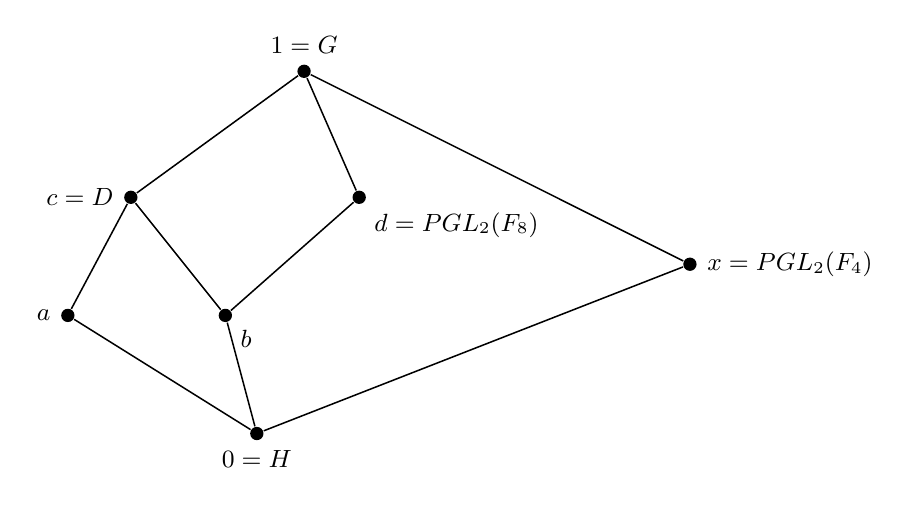
\begin{tikzpicture}[
    x=1cm,y=1cm,
    lattice point/.style={circle,fill,inner sep=1.7pt},
    every label/.style={font=\small},
    line width=0.55pt
  ]
    \node[lattice point,label=below:{$0=H$}] (zero) at (0,0) {};
    \node[lattice point,label=left:{$a$}] (a) at (-2.4,1.5) {};
    \node[lattice point,label=below right:{$b$}] (b) at (-0.4,1.5) {};
    \node[lattice point,label=left:{$c=D$}] (c) at (-1.6,3) {};
    \node[lattice point,label=below right:{$d=\operatorname{PGL}_2(\mathbb F_8)$}]
      (d) at (1.3,3) {};
    \node[lattice point,label=right:{$x=\operatorname{PGL}_2(\mathbb F_4)$}]
      (x) at (5.5,2.15) {};
    \node[lattice point,label=above:{$1=G$}] (one) at (0.6,4.6) {};
    \draw (zero)--(a)--(c)--(one)
          (zero)--(b)--(c)
          (b)--(d)--(one)
          (zero)--(x)--(one);
  \end{tikzpicture}
  \caption{The lattice $L_7$ realized as the subgroup interval $[H,G]$,
    where $G=\operatorname{PGL}_2(\mathbb F_{64})$ and
    $H=\operatorname{PGL}_2(\mathbb F_2)$. The group $D$ is the
    dihedral eigenpair stabilizer of order $126$; its subgroups $a$ and $b$
    containing $H$ have orders $42$ and $18$, respectively. Among the five
    interior elements, the only strict comparabilities are
    $a<c$, $b<c$, and $b<d$.}
  \label{f:fig-l7}
\end{figure}
